\chapter{Results}
\label{ch:results}
% -----------------------------------------------------------------------------

The goals of the project were to create a prototype, which response to the requirements specified in the specification.

\section{Control and read the uBoma}
\label{ch:results:control}

The first goal was to control the uBoma with the Rapsberry Pi.
To do that, it was necessary to be able to interact with the three devices.


\subsection{Rotary valve}
\label{ch:results:control:rotary}

Now, the rotary valve can be moved from end to end.
The client application offer the possibility to move the valve to any position and to display the current position.
The valve offer other possibility that are not implemented in the client application or in the core application but the class \texttt{RVM} is ready to be extended.
There is no magic character in the command and a new command can be added easily.
The figure \ref{ch:results:control:rotary:figure} show the card of the rotary valve.

\begin{figure}[H]
    \centering
    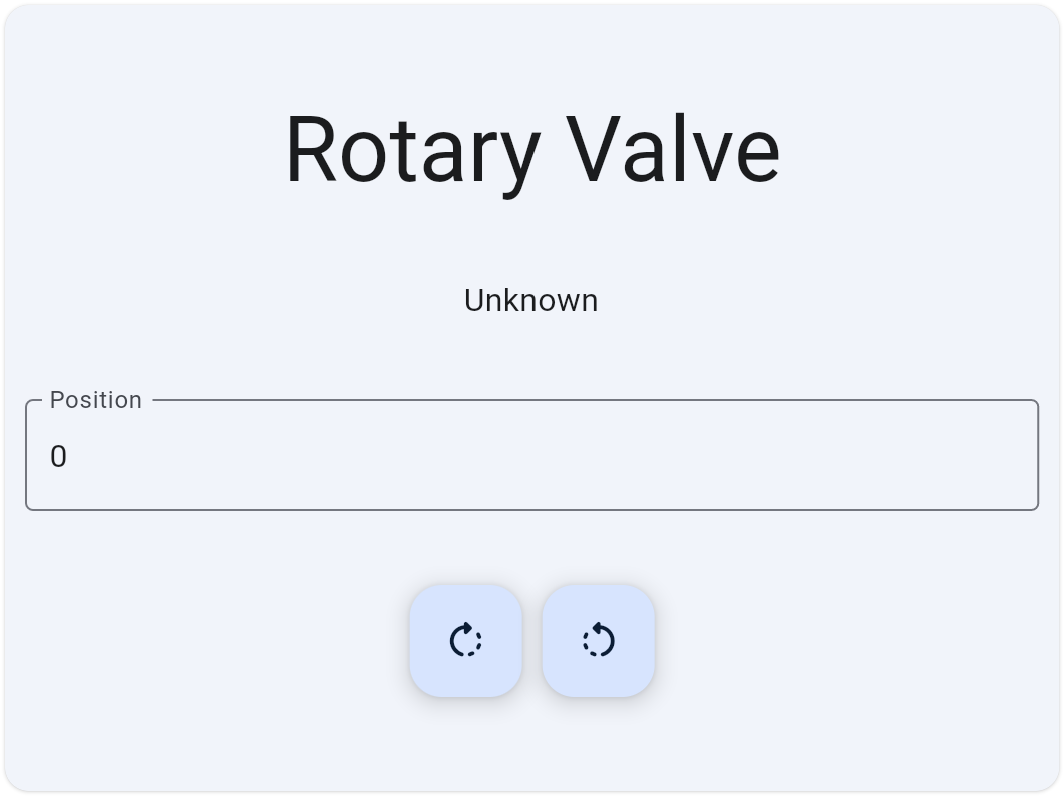
\includegraphics[width=0.5\textwidth]{img/results_rotary-card.png}
    \caption{Card of the rotary valve}
    \label{ch:results:control:rotary:figure}
\end{figure}

\subsection{Pressure sensor}
\label{ch:results:control:pressure}

The pressure sensor can be read and the value is displayed in the client application.
There is no control offered but some value to set the range of the sensor could be added in the future.

\subsection{Pressure controller}
\label{ch:results:control:controller}

The pressure controller isn't implemented yet.
The goal is to set the goal pressure and show the status of the controller.


\section{Provide an interface to the uBoma}
\label{ch:results:interface}

The second goal was to provide an interface to the uBoma.
The interface must be usable in a production and laboratory environment.

\subsection{Laboratory environment}
\label{ch:results:interface:laboratory}

At the end, the solution of a mobile application with Bluetooth was chosen.
This solution is a good end to end solutions for the laboratory environment because it's easy to use for the client.
The weak point of this solution is the deployment of the application.
The application must be installed on the device and it's more difficult to provide on an app store than a web application.

The second option is a web application.
This solution is easier to develop and to deploy.
The interaction between a client and a server through a REST API and web socket is easier to implement than a Bluetooth communication.
To deploy a web application, it's less complicated because it doesn't need to be accepted by an app store.
The weak point is that the web application must be reachable by the client.
The goal is to use the Raspberry Pi as a modem and to connect a client host through the wifi of the Raspberry Pi.

This second solution was implemented and the client application is developed with Flutter.
This is a framework based on Dart and it's possible to compile the application for Android, iOS, Windows, Linux and MacOS.
This is a good point and it allows us to not close the door to a mobile application in the future.
The figure \ref{ch:results:interface:laboratory:figure} show the client application.

\begin{figure}[H]
    \centering
    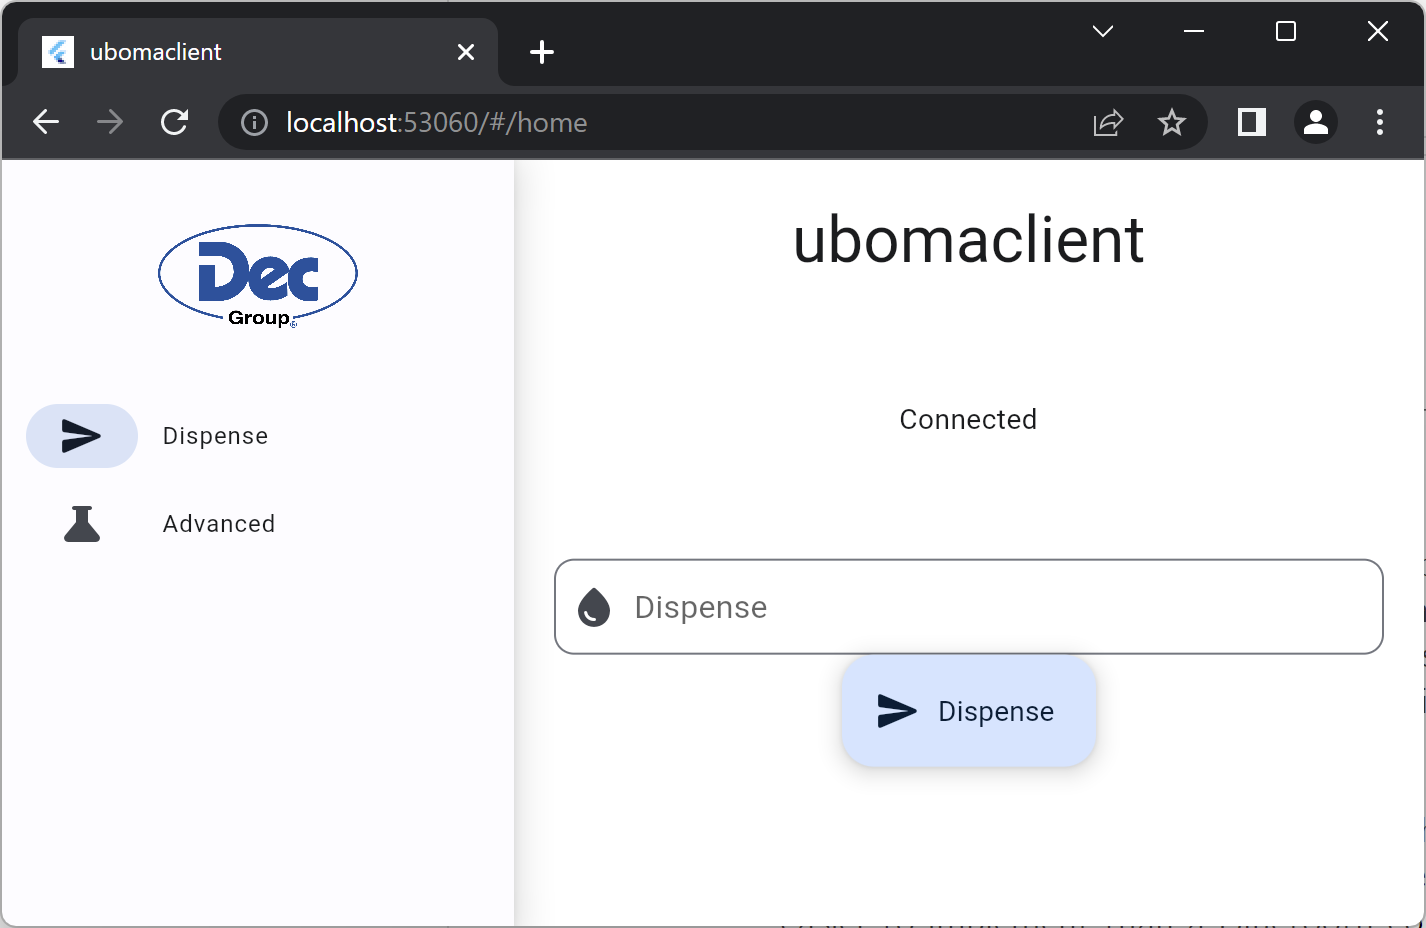
\includegraphics[width=0.75\textwidth]{img/results_clientApp.png}
    \caption{Client application}
    \label{ch:results:interface:laboratory:figure}
\end{figure}


\subsection{Production environment}
\label{ch:results:interface:production}

A second interface needs to be developed for the production environment.
The goal is to make uBoMa controllable by a central computer.
This interface must implement the protocol \acrfull{opc}, this is a standard protocol for industrial communication.
The \acrshort{opc} protocol is based on a client-server architecture and it must be implemented on the Ethernet port of the Raspberry Pi.
It's a must-have if the production requirement meets the \acrfull{mtp} and SilA standard.

This part was the next step after the laboratory application and it was not implemented yet.
The goal when this part will be implemented is just to add a new interface and keep the same action than the laboratory application.
